\documentclass[border=4pt]{standalone}

\usepackage{amsmath}
\usepackage{tikz}
\usepackage{mathdots}
\usepackage{yhmath}
\usepackage{cancel}
\usepackage{color}
\usepackage{siunitx}
\usepackage{array}
\usepackage{multirow}
\usepackage{amssymb}
\usepackage{gensymb}
\usepackage{tabularx}
\usepackage{booktabs}
\usetikzlibrary{fadings}
\usetikzlibrary{patterns}


\begin{document}
 



\tikzset{every picture/.style={line width=0.75pt}} %set default line width to 0.75pt        

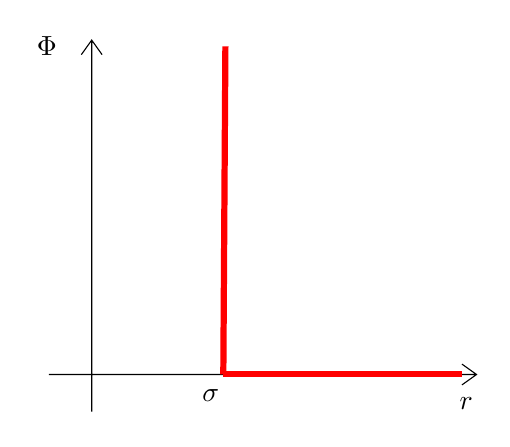
\begin{tikzpicture}[x=0.75pt,y=0.75pt,yscale=-1,xscale=1]
%uncomment if require: \path (0,300); %set diagram left start at 0, and has height of 300

%Shape: Axis 2D [id:dp85144241619174] 
\draw  (50,244.1) -- (256,244.1)(70.6,83) -- (70.6,262) (249,239.1) -- (256,244.1) -- (249,249.1) (65.6,90) -- (70.6,83) -- (75.6,90)  ;
%Straight Lines [id:da3273427167193963] 
\draw [color={rgb, 255:red, 255; green, 0; blue, 0 }  ,draw opacity=1 ][line width=2.25]    (135,86) -- (134,244) ;


%Straight Lines [id:da8623763519234107] 
\draw [color={rgb, 255:red, 255; green, 0; blue, 0 }  ,draw opacity=1 ][line width=2.25]    (134,244) -- (249,244) ;



% Text Node
\draw (251,258) node    {$r$};
% Text Node
\draw (49,86) node    {$\Phi $};
% Text Node
\draw (128,254) node    {$\sigma $};


\end{tikzpicture}

\end{document}
